\documentclass[tikz,border=12pt]{standalone}
\usepackage[T1]{fontenc}
\usepackage{tgheros}
\usepackage{sfmath}
\usepackage{amsmath}
\usepackage{fontawesome5}
\usepackage{tikz}
\usetikzlibrary{arrows.meta,positioning,shapes.geometric,fit,backgrounds,calc}
\usepackage{xcolor}

\renewcommand{\familydefault}{\sfdefault}

% Harvard Crimson & ETH Zurich Academic Semantic Palette
\definecolor{harvardcrimson}{HTML}{A51C30}
\definecolor{ethdarkblue}{HTML}{1F407A}
\definecolor{ethblue}{HTML}{215CAF}
\definecolor{ethpetrol}{HTML}{007A87}
\definecolor{ethbronze}{HTML}{B87333}
\definecolor{ethpurple}{HTML}{5B4B8A}
\definecolor{ethslate}{HTML}{475569}
\definecolor{cardbg}{HTML}{F8FAFC}
\definecolor{cardborder}{HTML}{CBD5E1}
\definecolor{notbind}{HTML}{EEF1F5}

\begin{document}
\begin{tikzpicture}[
  font=\sffamily,
  >=Stealth,
  x=1.62in, y=-0.86in,
  cell/.style={
    draw=cardborder, fill=white, line width=0.6pt,
    minimum width=1.58in, minimum height=0.80in,
    text width=1.44in, align=center, inner sep=3pt, anchor=center
  },
  dominant/.style={cell, line width=1.5pt, fill=cardbg},
  thin/.style={cell, fill=white},
  nobind/.style={cell, fill=notbind, draw=cardborder!70},
  colhead/.style={
    draw=none, fill=none, minimum width=1.58in, text width=1.48in,
    align=center, anchor=center, inner sep=2pt
  },
  rowhead/.style={
    draw=ethdarkblue, fill=ethdarkblue!8, rounded corners=4pt, line width=0.9pt,
    minimum width=1.35in, minimum height=0.80in, text width=1.22in,
    align=center, anchor=center, inner sep=3pt
  }
]

% ---------- Title ----------
\node[draw=ethdarkblue, fill=ethdarkblue!5, rounded corners=5pt, line width=1pt,
      text width=9.55in, inner sep=7pt, align=center, anchor=center] at (2.0, -1.62) {
  {\normalsize\bfseries\color{ethdarkblue}\faIcon{th}\;\; THE PHYSICAL AI CO-DESIGN MATRIX}\\[2pt]
  {\scriptsize\color{ethslate}Twenty-five questions. Five cognitive obligations against five physical constraints. Part II answers them one row at a time.}
};

% ---------- Column headers ----------
\node[colhead] at (0,-0.82) {{\scriptsize\bfseries\color{ethblue}Time \&\\Freshness}};
\node[colhead] at (1,-0.82) {{\scriptsize\bfseries\color{ethbronze}Inertia \&\\Stopping}};
\node[colhead] at (2,-0.82) {{\scriptsize\bfseries\color{harvardcrimson}Actuation\\Limits}};
\node[colhead] at (3,-0.82) {{\scriptsize\bfseries\color{ethpurple}Energy \&\\Thermal}};
\node[colhead] at (4,-0.82) {{\scriptsize\bfseries\color{ethpetrol}Silicon\\Determinism}};

% ---------- Row headers ----------
\node[rowhead] at (-1.02,0) {{\scriptsize\bfseries PERCEIVE}\\[1pt]{\tiny\color{ethslate}Ch 4 \textperiodcentered\ \texttt{OBS-01}}};
\node[rowhead] at (-1.02,1) {{\scriptsize\bfseries REMEMBER}\\[1pt]{\tiny\color{ethslate}Ch 5 \textperiodcentered\ \texttt{STATE-01}}};
\node[rowhead] at (-1.02,2) {{\scriptsize\bfseries REASON}\\[1pt]{\tiny\color{ethslate}Ch 6 \textperiodcentered\ \texttt{INTENT-01}}};
\node[rowhead] at (-1.02,3) {{\scriptsize\bfseries PLAN}\\[1pt]{\tiny\color{ethslate}Ch 7 \textperiodcentered\ \texttt{PLAN-01}}};
\node[rowhead] at (-1.02,4) {{\scriptsize\bfseries EXECUTE}\\[1pt]{\tiny\color{ethslate}Ch 8 \textperiodcentered\ \texttt{ENF-01}}};

% ---------- Row 1: Perceive ----------
\node[thin]      at (0,0) {{\tiny When did this\\observation happen?}};
\node[thin]      at (1,0) {{\tiny How far ahead\\must you see?}};
\node[nobind]    at (2,0) {{\tiny\itshape\color{ethslate}not binding}\\[1pt]{\tiny\color{ethslate}commands nothing}};
\node[thin]      at (3,0) {{\tiny What does sensor heat\\do to geometry?}};
\node[dominant, draw=ethpetrol] at (4,0) {{\tiny\bfseries\color{ethpetrol}DOMINANT}\\[1pt]{\tiny What does moving\\the pixels cost?}};

% ---------- Row 2: Remember ----------
\node[dominant, draw=ethblue] at (0,1) {{\tiny\bfseries\color{ethblue}DOMINANT}\\[1pt]{\tiny What is a belief\\worth after $\Delta t$?}};
\node[thin]      at (1,1) {{\tiny How much world\\must you hold?}};
\node[thin]      at (2,1) {{\tiny\itshape\color{ethslate}thin}\\[1pt]{\tiny relocalization snap}};
\node[thin]      at (3,1) {{\tiny Which calibration\\drifts with heat?}};
\node[thin]      at (4,1) {{\tiny Bounded state\\without allocation}};

% ---------- Row 3: Reason ----------
\node[dominant, draw=ethblue] at (0,2) {{\tiny\bfseries\color{ethblue}DOMINANT}\\[1pt]{\tiny How long may intent\\outlive its world?}};
\node[nobind]    at (1,2) {{\tiny\itshape\color{ethslate}not binding}\\[1pt]{\tiny reaches via the lease}};
\node[nobind]    at (2,2) {{\tiny\itshape\color{ethslate}not binding}\\[1pt]{\tiny commands no torque}};
\node[thin]      at (3,2) {{\tiny What does throttling\\do to a deadline?}};
\node[thin]      at (4,2) {{\tiny Keeping a large model\\off the real-time core}};

% ---------- Row 4: Plan ----------
\node[thin]      at (0,3) {{\tiny Outliving the latency\\that produced it}};
\node[thin]      at (1,3) {{\tiny What makes a plan\\abandonable?}};
\node[dominant, draw=harvardcrimson] at (2,3) {{\tiny\bfseries\color{harvardcrimson}DOMINANT}\\[1pt]{\tiny What shapes may\\a command take?}};
\node[thin]      at (3,3) {{\tiny What does a motion\\cost per shift?}};
\node[thin]      at (4,3) {{\tiny\itshape\color{ethslate}thin}\\[1pt]{\tiny compute as a budget}};

% ---------- Row 5: Execute ----------
\node[thin]      at (0,4) {{\tiny The deadline, and the\\cycle it is missed}};
\node[dominant, draw=ethbronze] at (1,4) {{\tiny\bfseries\color{ethbronze}DOMINANT}\\[1pt]{\tiny How much margin\\does stopping need?}};
\node[thin]      at (2,4) {{\tiny Can the veto violate\\the limit it protects?}};
\node[thin]      at (3,4) {{\tiny What clamps the\\current asked for?}};
\node[thin]      at (4,4) {{\tiny Code that may\\never pause}};

% ---------- Legend ----------
\node[draw=ethdarkblue, fill=white, rounded corners=4pt, line width=0.8pt,
      text width=9.55in, inner sep=6pt, align=center, anchor=center] at (2.0, 4.92) {
  {\scriptsize\textbf{\color{ethdarkblue}READING THE GRID:}\;
  \textbf{Bold border} marks each chapter's dominant cell, where most of its length goes.\;
  \textbf{Shaded} cells do not bind, and saying why is part of the argument.\;
  The grid is uneven because the physics is.}
};

\end{tikzpicture}
\end{document}
